\documentclass[review,nonacm,screen,acmsmall,anonymous=true]{acmart}
\settopmatter{printfolios=true,printccs=true,printacmref=true}

\bibliographystyle{ACM-Reference-Format}
\citestyle{acmauthoryear}   %% For author/year citations
\usepackage{mathpartir}
\usepackage[utf8]{inputenc}
\usepackage{fontenc}
\usepackage{microtype}
\usepackage{listings,array,multirow,wrapfig,xspace,booktabs,subcaption}
\usepackage{xcolor,tikz, graphicx, pifont}
\usetikzlibrary{positioning}

\newcommand{\authorcomment}[3]{\xspace\textcolor{#1}{{\bf #2} #3}\xspace}
% For author notes:
\newcommand{\AG}[1]{\authorcomment{orange}{AG}{#1}}
\newcommand{\JV}[1]{\authorcomment{red}{JV}{#1}}
\newcommand{\JJ}[1]{\authorcomment{green}{JJ}{#1}}
\newcommand{\SK}[1]{\authorcomment{yellow}{SK}{#1}}
\newcommand{\OF}[1]{\authorcomment{magenta}{OF}{#1}}

% For meta comments:
\newcommand{\isit}[1]{\authorcomment{cyan}{Check}{#1}}
\newcommand{\todo}[1]{\authorcomment{red}{TODO}{#1}}
\newcommand{\xmark}{\color{red} \ding{55}}
\newcommand{\cmark}{\color{green} \ding{51}}

\newcommand{\always}{\emph{Always}\xspace}
\newcommand{\sometimes}{\emph{Sometimes}\xspace}
\newcommand{\sometimesStar}{\emph{Sometimes*}\xspace}
\newcommand{\never}{\emph{Never}\xspace}
\newcommand{\neverStar}{\emph{Never*}\xspace}

\lstset{language=R}

\definecolor{LightGray}{RGB}{247, 247, 247}
\definecolor{Gray}{rgb}{.3,.3,.3}
\definecolor{DarkGray}{rgb}{.5,.5,.5}

\lstset{ %
  columns=flexible,
  captionpos=b,
  frame=single,
  framerule=0pt,
  framexleftmargin=1mm,
  framexrightmargin=1mm,
  tabsize=2,
  belowskip=0pt,
  basicstyle=\small\ttfamily,
  backgroundcolor=\color{LightGray},
  emphstyle=\sffamily,
  keywordstyle=\bfseries,
  commentstyle=\color{Gray}\em,
  stringstyle=\color{Gray}
}
\lstdefinestyle{R}{ %
  language=R,
  deletekeywords={new, env, equal, c, runif, trace, args, exp, t, all, get,
    names, is, environment, class, substitute, expression, list, null, Internal,
    sample, diag, length, rep, nrow, stop, offset, pmax, Machine,
    double, parent, frame, par, methods, end, dir, apply, deparse, missing,
    plot, as, integer, character, inherits, numeric, paste, eval, quote, call,
    formula, df, log, sum, c, local, legend, file, scale, round, title, order,
    drop, which, grid, print, ncol, dim, max, format, sort, rug, matrix, start,
    unique, mean, df, attr, do, power},
  otherkeywords={},
  breaklines=true
}

\newcommand{\code}[1]{\lstinline[style=R]|#1|\xspace}
\renewcommand{\c}[1]{\lstinline[style=R]|#1|\xspace}
\newcommand{\lazr}{\emph{lazr}}
\newcommand{\strictr}{\emph{strictr}}

%% Performance evaluation results:

\newcommand{\benchmarkSuiteSize}{14\xspace}

%% Baseline perf  Gnur - Rsh (1x15)  
%% https://rir-benchmarks.prl.fit.cvut.cz/diff?warmup=5&kind=diff&job_ids%5B%5D=1169772175&job_ids%5B%5D=1169772178&selection=promisebreaker
\newcommand{\speedupRsh}{$1.89\times$\xspace}
\newcommand{\speedupRshMax}{$56\times$\xspace}
\newcommand{\speedupRshMin}{$0.64\times$\xspace}

%%  Speedup  Rsh - Rsh strict (4x25)  
%% https://rir-benchmarks.prl.fit.cvut.cz/diff?warmup=5&kind=diff&job_ids%5B%5D=1174881563&job_ids%5B%5D=1174869738&execution=all&selection=promisebreaker
\newcommand{\speedupRshStrict}{$1.17\times$\xspace}
\newcommand{\speedupRshStrictMax}{$1.95\times$\xspace}
\newcommand{\speedupRshStrictMin}{$0.92\times$\xspace}
\newcommand{\speedupRshStrictSignificant}{9\xspace}  %% *** TODO: WHAT DOES SIGNIFICANT MEAN? **

%%  Speedup BC  (1x15) 
%% https://rir-benchmarks.prl.fit.cvut.cz/diff?warmup=5&kind=diff&job_ids%5B%5D=1172677834&job_ids%5B%5D=1172663147&selection=promisebreaker
\newcommand{\speedupBCRshStrict}{$1.16\times$\xspace}
\newcommand{\speedupBCRshStrictMax}{$1.48\times$\xspace}
\newcommand{\speedupBCRshStrictMin}{$1.00\times$\xspace}

%%  How much is BC slower?
%% https://rir-benchmarks.prl.fit.cvut.cz/diff?warmup=5&kind=diff&job_ids%5B%5D=1174869738&job_ids%5B%5D=1172663147&execution=all&selection=promisebreaker
\newcommand{\rshBCSlowdown}{$0.38\times$\xspace}

%% Reduction in promise allocation:
%% promise numbers using 1x15 iterations
\newcommand{\promiseAlocationReductionGnurRsh}{$91\%$\xspace}  %% 91.3 
\newcommand{\promiseAlocationReductionRshStrict}{$96\%$\xspace}  %%   95.6  OK (excluding fastaredux and fannkuchredux)
\newcommand{\promiseAlocationReductionGnurRshStrict}{$99\%$\xspace}   %%  99.33  (excluding fastaredux and fannkuchredux) 
\newcommand{\promiseAlocationReductionRshStrictToZero}{$2$\xspace}  %% OK (fastaredux and fannkuchredux drop to 0)
\newcommand{\promiseAlocationReductionGnurRshStrictMin}{$9.5\%$\xspace}  %% OK

%% time in GC in  Ř-strict / time in GC in Ř
\newcommand{\speedupGCRshStrictMax}{$190\%$\xspace}
\newcommand{\speedupGCRshStrictMin}{$50\%$\xspace}

%% How much is due to reduced allocation
%% https://rir-benchmarks.prl.fit.cvut.cz/diff?warmup=5&kind=diff&job_ids%5B%5D=1183876408&job_ids%5B%5D=1172677834&job_ids%5B%5D=1172663147&selection=promisebreaker
\newcommand{\speedupBCRshStrictAlloc}{$1.1\times$\xspace}
\newcommand{\speedupDueToReducedGC}{$38\%$\xspace}


\newcommand{\robustnesResult}{$0.56\%$\xspace}


%%% \setcopyright{rightsretained}
%%% \acmPrice{}
%%% \acmDOI{10.1145/3360579}
%%% \acmYear{2019}
%%% \copyrightyear{2019}
%%% \acmJournal{PACMPL}
%%% \acmVolume{3}
%%% \acmNumber{OOPSLA}
%%% \acmArticle{153}
%%% \acmMonth{10}
\begin{document}
\title{Promises Are Made To Be Broken}
\subtitle{Migrating the R ecosystem to strict evaluation semantics}

\author{Aviral Goel}\affiliation{\institution{Northeastern University}\country{USA}}
\author{Jan Ječmen}\affiliation{\institution{Czech Technical University}\country{Czechia}}
\author{Sebastián Krynski}\affiliation{\institution{Czech Technical University}\country{Czechia}}
\author{Oliver Flückiger}\affiliation{\institution{Northeastern University}\country{USA}}
\author{Jan Vitek}\affiliation{\institution{Czech Technical University and Northeastern University}\country{USA}}
\authorsaddresses{}
\renewcommand{\shortauthors}{Goel, Vitek}

\begin{abstract}
  Function calls in the R language do not evaluate their arguments; these are
  passed as suspended computations to the callee which evaluates them only if
  they are needed. After 25 years of experience with the language, there are
  very few cases where programmers leverage delayed evaluation intentionally.
  Yet being lazy comes at a price in performance and complexity. This paper
  explores how one could evolve the semantics of the language towards strictness
  by default and laziness on demand. To provide a migration path, it is
  necessary to change the semantics of the language implementations and provide
  tooling for developers to migrate the libraries and user code in a way that
  does not introduce errors. This paper reports on a dynamic analysis that
  infers strictness signatures for functions and capture both intentional and
  accidental laziness. To assess the robustness of the inferred signatures, we
  implemented a source-to-source refactoring that forces the evaluation of
  arguments that have been annotated as strict. Finally, we report on the
  performance benefits of migration by extending a just-in-time compiler with
  support for strictness annotations.
\end{abstract}

\begin{CCSXML}
<ccs2012>
<concept>
<concept_id>10002944.10011123.10010912</concept_id>
<concept_desc>General and reference~Empirical studies</concept_desc>
<concept_significance>500</concept_significance>
</concept>
<concept>
<concept_id>10011007.10011006.10011008</concept_id>
<concept_desc>Software and its engineering~General programming languages</concept_desc>
<concept_significance>500</concept_significance>
</concept>
<concept>
<concept_id>10011007.10011006.10011050.10010517</concept_id>
<concept_desc>Software and its engineering~Scripting languages</concept_desc>
<concept_significance>500</concept_significance>
</concept>
<concept>
<concept_id>10011007.10011006.10011039.10011311</concept_id>
<concept_desc>Software and its engineering~Semantics</concept_desc>
<concept_significance>300</concept_significance>
</concept>
</ccs2012>
\end{CCSXML}

\ccsdesc[500]{General and reference~Empirical studies}
\ccsdesc[500]{Software and its engineering~General programming languages}
\ccsdesc[500]{Software and its engineering~Scripting languages}
\ccsdesc[300]{Software and its engineering~Semantics}

\keywords{R language, delayed or lazy evaluation}

\maketitle
\section{Introduction}

The R programming language is widely used in data science. Unbeknownst to many
of its end-users, function calls have a call-by-need, or lazy, semantics. In
other words the arguments of a function call are suspended computations which
are evaluated if and when they are needed. \citet{oopsla19b} provided a thorough
observational study of a corpus consisting of 16,707 packages written in R. For
the most part, the corpus appears to have been written without reliance on
laziness with the exception of code that leverages it for meta-programming.

This paper argues that laziness should be the exception in R. We propose to make
it a \emph{eager by default, lazy on demand} language by introducing strictness
annotations. The question we wish to answer is whether it is possible to switch
the semantics of a language without causing undue breakage in the legacy code
that is in daily use. This concern is relevant because, even if programmers
don't avail themselves of call-by-need, it is conceivable that their code
accidentally depends on it. A change in the order of evaluation of arguments may
introduce errors if that code was performing side effects.

\paragraph{The Case for Strictness.} Laziness is error-prone, inconsistent
and costly. The combination of delayed evaluation and side-effects in a language
without type annotations is an invitation to subtle programming errors. If a
function has multiple evaluation orders and is called with effectful arguments,
their effects will be observed to happen in various orders. Functional languages
prevent ordering issues by reflecting effects in the type system. R cannot do
this as it is dynamically typed. Instead, libraries routinely add code at the
boundaries of their API to force a single evaluation order. The design and use
of call-by-need is inconsistent because there are multiple points where
evaluation is arbitrarily forced. These include right-hand side of assignments
and function returns, neither of which is required in a lazy language.
Furthermore, to support object-oriented programming, R allows both single- and
multiple-dispatch; in order to perform dispatch, arguments must be evaluated
eagerly. Last, there are costs to lazy evaluation. Each argument must be boxed
in a data structure that holds a reference to the expression to evaluate, its
environment and the result of evaluation. Allocating and deallocating these data
structures put pressure on the memory manager. Delayed evaluation further
complicates the work of compilers for the language by hindering optimizations
and increasing the number of indirect calls.

\paragraph{The Case for Laziness.} The success of a programming language
often comes down to the strength of its ecosystem. With tens of millions of
lines of contributed library code, any change to the core semantics of the
language risks changing the behavior of some library functions. Preserving the
status quo is a pragmatic choice to protect the investment in legacy code bases.
Laziness is needed for an additional reason, it is the building block of the
meta-programming facilities of the language. Unevaluated arguments can be
coerced back to their source code, that code can be modified, and evaluated in
an environment of the programmer's choice. Meta-programming is used to extend
the language and to create embedded domain specific languages. While it is
possible to imagine using macros instead, the number of libraries that use
meta-programming is sufficiently large that it would be non-trivial to refactor
them.

\section{Background}

This section sets the stage by introducing related work and giving a brief
overview of R.

\subsection{Related Work}

There are three clusters of related results: research on adding and removing
laziness in functional languages, research on the R language, and approaches to
language migration.

\paragraph{Call by need}  Functional languages with
a call by need evaluation strategy must contend with memory pressure and
associated performance issues due to allocation of substantial numbers of thunks
(suspended computations)~\cite{transformopt,stricteffective,opteval}. While most
Haskell programs benefit from the strictness analysis pass performed by the
compiler. Due to its conservative nature, this pass misses some opportunities
for optimizations. To recover performance programmers can manually insert
strictness annotations to control evaluation but identifying where to put them
can be challenging. \citet{autobahn} proposed, Autobahn, a tool that
automatically infers strictness annotations using a genetic algorithm. The
approach relies on a dynamic analysis, as it does not approximate and cannot
guarantee termination on all inputs. As the annotations are based on a
heuristic, developers must manually validate their soundness. The authors report
an average 8.5\% speedup (with a maximum speed up of 89\%). \citet{lazyprof}
solve the complementary problem of suggesting laziness annotations for
call-by-value $\lambda$ calculus using a dynamic analysis. They introduce the
notion of laziness potential, a predictor of the benefit obtained by making an
expression lazy. They use this as a guide to insert laziness annotations. They
demonstrate benefits on Racket implementations of Okasaki's purely functional
data structures, monadic parser combinators, and an AI game. The present paper
is similar to Autobahn in that we infer annotations dynamically and we do not
guarantee soundness. Where our work departs from Autobahn is that we use
execution traces to determine strictness. Furthermore, we have to deal with
side-effects and reflective operations, they introduce extra complexity for our
synthesis algorithm.

\paragraph{The R language} \citet{oopsla19b} investigated the design and use of
laziness in R. They provide a detailed account of the language's evaluation
strategy with a small-step operational semantics and an empirical evaluation of
laziness in 16,707 packages. Their study shows that most R code is written
without reliance on, or awareness of, laziness. Out of 388K functions, 83\%
evaluate all of their arguments in a single order across all calls. The authors
found that programmers sometime force evaluation of arguments at the beginning
of a function to protect their code from non-deterministic effects. Only a
single instance of a lazy data structure could be found. The main \emph{raison
d'\^etre} for delayed evaluation seems to be meta-programming. \citet{oopsla20b}
empirically inferred type signatures for functions by dynamically observing the
type of arguments and return values. The authors validated these signatures by
inserting type checking code inside functions and monitor type failures on
client programs. This approach inspired our strictness inference, but types are
easier to check for soundness than strictness. For types, one simply inserts
code that checks that, if an argument is eventually evaluated, it evaluates to
the expected type. For strictness, we have to worry about the interplay of
side-effects and changes to the order of evaluation of arguments. This makes
validation of strictness signatures hard.

\paragraph{Language migration}
With this work, we are trying to propose a change in the semantics of R. The
most prominent contemporary example is the transition from Python 2 to Python 3,
which is still ongoing. Python 3 was released in 2008 with many incompatible
changes. The plan \cite{pysunset} to drop support for Python 2 was postponed
from 2015 to 2020 since a lot of codebase was not transitioned to Python 3.
Currently, the translation has been mostly automated by tools such as
\emph{Futurize}, and \emph{py2to3}.

\AG{Do we want to talk about PHP-Hack and JS strict mode?}

ADD: Gradual typing

ADD: Typescript


\subsection{The R Language}

\subsection{Missingness}

A function in R can be called with fewer arguments than expected. These
argumentless parameters are treated as missing if they don't have a default
value. The function can check for missing arguments using the \code{missing}
function. Since missing arguments can be forwarded to callees, \code{missing}
performs this check transitively. The strictness signatures we compute reflect
the function's strictness with respect to its arguments when they are not
missing.


\subsection{Metaprogramming}
The \code{substitute} function provides reflective access to an argument's
unevaluted code contained inside the promise. This can also be done in native
code using the \code{PREXPR} C macro on the promise object. These cases reflect a
genuine use of laziness. Functions are treated as lazy in these arguments, even
if the arguments are evaluated.

\subsection{Reflection}
R provides reflective access to its first class environments and it

\subsection{Effects}

\subsection{Vararg}
varargs, or $...$ paramaters, accept an arbitrary number of arguments, including
missing arguments. The function can materialize $...$ into a list using the
\code{list(...)} pattern. This saves the user from packaging the arguments into
a list. The function can also forward its $...$ to a callee. This enables the
function to expose its callee's interface to the callers without listing
callee's parameters and their default values.


\section{Strictness Signatures}

A function's strictness signature is a tuple $\langle f, s_1, ..., s_n \rangle$,
where $f$ is the function's qualified name and $s_i$ are positions of arguments
that can be evaluted strictly. We synthesize these signatures from dynamically
generated traces. There are many language ``features'' the affect the decision
to evaluate an argument eagerly.

Arguments used for metaprogramming using \code{substitute} and \code{PREXPR} are
never strict. The code is reflectively accessing the unevaluated argument text
from these argument promises. Eliminating these promises will break this part of
the code.

$...$ arguments are always treated as lazy. Assigning a single strictness
annotation to $...$ is tricky because a function can have different strictness
behavior for the individual arguments of $...$. One solution is to treat the
function strict in $...$ if it is strict in all of its constituents. However,
this signature may still not be unique. Unlike normal argument promises,
promises inside $...$ are not packaged in a new promise but rather forwarded
as-is to callees. A function's callees may use metaprogramming on the promises
inside $...$ even if the function itself does not . Furthermore, a $...$ passed
to a callee could be forwarded further down resulting in a long chain of
functions having access to the same argument promises. All these functions in
the chain can directly affect these arguments. The presence of missing arguments
inside $...$ introduces another wrinkle.

An argument may not be evaluated in all calls to the function. This means the
function function is not strict in that argument. Unless the documentation
dictates that this argument is evaluated in special cases where it is expected
to perform a reflective or effectful operation, we could still evaluate it
without any observable consequence except a performance penalty.

Functions \code{as.environment} and \code{pos.to.env} when invoked with argument
\code{-1} return the environment of the parent call on the stack. Calling them
directly from inside a promise makes the promise's result sensitive to the frame
of its evaluation. Forcing this argument promise eagerly on function entry could
result in a different result if the promise was being passed down to callees for
evaluation in the original program. This makes the function lazy in that
argument even if its implementation does not require this argument to be lazy.
This code has an accidental reliance on laziness. If the function's
documentation does not make any commitment about the frame in which this
argument will be evaluated, this code will be susceptible to breakage due to
change in the function's implementation.

Arguments can perform side-effects. Many argument promises will contain a symbol
referring to the value being passed as the argument, so they will at least
perform a read in the caller's environment. Similarly, some promises contain
function call expressions which will do local writes in the environment created
for the function call during promise evaluation. These effects are benign and do
not affect our decision to evaluate the corresponding arguments strictly.
However, if a promise writes to the caller's environment, or more generally, to
any environment that is not created during its evaluation, then that write is
observable by code outside the promise. Also, if a promise reads from an
environment that is modified after the promise is created and before it is
evaluated, then that argument should also be treated lazily. Arguments that
perform these reads and writes depend on the evaluation order implemented by the
function to which they are passed. Unless the function's documentation describes
this order, these uses are wrong. A change in function's implementation could
cause the reads and writes to happen in a different order, or not at all,
leading to incorrect results. Similarly, errors are another source of effect
inside promises. They can either stop the program execution or be captured by an
enclosing exception handler.

Use of metaprogramming and $...$ arguments are \emph{intrinsic} factors
affecting a function's strictness. On the other hand, passing side-effecting
arguments or arguments with reflective calls, especially in argument positions
that may not be always evaluated makes the function's strictness dependent on
how it is used. These are \emph{extrinsic} factors with an accidental reliance
on laziness. In our experiments $...$ and metaprogrammed arguments are always
treated as non-strict. In contrast to side-effecting and reflective promises
these are genuine uses of laziness as they are not affected by the client. With
this as the base amount of laziness, we could try to evaluate the rest of
arguments in different combinations. A combination of these choices results in
many possible signature configurations. We discuss them in detail in the
\nameref{Evaluation:Robustness} section.

\section{Analysis Infrastructure}
In this section, we describe our analysis pipeline that \emph{(a)} synthesizes
strictness signatures from execution traces, \emph{(b)} validates them by
enforcing strict argument evaluation, and \emph{(c)} analyzes execution traces
for insights. Our experiments were performed on two Intel Xeon 6140, 2.30GHz
machines with 72 cores and 256GB of RAM each. The analysis pipeline starts with
setting up a Docker image that includes all the dependencies for installing
analysis code and R packages from CRAN and Bioconductor. This provides a
reliable reproducible setup across the two machines. Next, we mirror CRAN and
Bioconductor\cite{bioc} repositories and install their R packages. This is
followed by generation of execution traces from a dynamic analyzer running
inside an instrumented R virtual machine. These traces are analyzed to generate
tabular data files and strictness signatures. Finally, the signatures are
applied to client programs for validation. The pipeline is managed by a Makefile
which has rules for every step. This makes it easy to administer the experiments
on multiple machines. Whenever possible, we parallelize the steps using GNU
parallel\cite{tange2011a}.

\subsection{Synthesizing Strictness Signatures}

For synthesizing strictness signatures, we observe the evaluation of arguments
from dynamically generated execution tracer. For this, we use an instrumented R
virtual machine, \emph{R-dyntrace} \citet{oopsla19b} based on GNU-R version
4.0.2. It exposes events for invoking user-defined callbacks with raw R object
at specific points inside the R interpreter. Extracting meaningful information
from these R objects at this low level requires handling a lot of subtleties
arising from the intricacies of R's execution model. These details are
surprisingly hard to get right. The challenges are described in detail by
\cite{oopsla19b} in the design of their tracer for collecting information about
use of laziness in R programs.

\AG{TODO: Add LOC for R-dyntrace and instrumentr}

To iron these wrinkles, we developed \emph{instrumentr}, an R package that
provides a layer of abstraction on top of the event framework exposed by
\emph{R-dyntrace}. \emph{instrumentr} provides an API to create tracer objects
to which event specific callbacks can be attached. \emph{instrumentr} intercepts
\emph{R-dyntrace} events and invokes the corresponding tracer's callbacks. It
passes model objects to callbacks by wrapping the raw R objects provided to its
own callbacks registered with \emph{R-dyntrace}. These model objects contain
metadata about the raw R object and provide a consistent API for inspecting
their constituents. The object metadata keeps track of the object's unique id.
This uniqueness guarantee enables downstream client analyses to key objects by
their id instead of addresses which are not unique since they get resused by R's
garbage collector. The model objects are reference counted which makes it
possible for a model object to be referenced by multiple model objects with
proper memory management. A complication arises in this design when objects have
cyclic references. For example, a promise argument keeps a reference to a call
object and vice-versa. To address this, \emph{instrumentr} defines the notion of
a primary owner. The primary owner of a model object can ``kill'' the object,
i.e. free up object's internals (and decrement the references it holds to other
objects) even if it is referenced by other objects. Killing does not free up the
model object's memory or affect its metadata. This lets secondary owners access
the dead object's metadata even after the raw R object no longer exists. The
``dead'' object's memory is finally freed when it is no longer referenced by any
other object in the system. This design insight makes it trivial to express
complex object dependencies without any memory leaks at the scale of millions of
objects. This also enables clients to query dead object's metadata if they are
referenced by model objects made available to the clients via their callbacks.
This greatly simplifies the handling of promises, first class environments and
function calls.

\emph{instrumentr} keeps track of logical time, from tracing
entry to tracing exit, incremented on every event. The model object's metadata
keeps track of its time of allocation and deallocation. For environments, it
also keeps track of last read and last write time. For promises, it keeps track
of force entry and force exit time. This information is used to identify
non-local reads and writes to environments.

For performance, \emph{instrumentr} caches model objects in a table keyed by the
R object's address. Table entries are inserted and erased on \emph{object
  allocation and deallocation} events respectively. This prevents duplication of
model objects when the same R object is encountered on multiple events.

\emph{instrumentr} models the call stack. It also adds promise objects under
evaluation to the stack. This helps identify if an event, say a side-effect, is
occuring inside a promise. Furthermore, R uses \emph{longjmp} to do non-local
returns. \emph{instrumentr} exposes a deterministic behavior during such events
by artificially calling the exit callbacks of interrupted calls and promises on
the stack. This simplifies the client side tracing logic, significantly.

\emph{instrumentr} keeps track of environment and function names in their model
objects. Getting fully qualified function names dynamically is challenging in R
because package namespaces are first class environments that are constructed
piecemeal and all functions are by default anonymous objects that may be bound
to a name in their lexical scope. \emph{instrumentr} handles this by assigning
names to environments on package load events and checking on every write if a
function is being bound to a name. Functions can be nested to arbitrary depths
in which case \emph{instrumentr} links model function objects to reflect the
parent-child relationship.

For extracting execution traces, we developed \emph{lazr}, an R library which
sits atop \emph{instrumentr}. \emph{lazr} collects information about function
calls, arguments, side-effects, and reflective environment access. from the
model objects provided by the following instrumentr event: \emph{function entry
  and exit}, \emph{promise evaluation entry and exit}, \emph{variable reads and
  writes}, \emph{promise value and expression reads}, and \emph{function
  lookup}. This information is stored in compressed tabular format using R's
\emph{fst} library.

For signature generation, we use a custom R script that summarizes argument
evaluation data per function from the tables generated by \emph{lazr} and
generates signatures for different strictness configurations. We generate one
file per package per signature configuration containing signatures for all
top-level functions of that package. Here is how the signature file for package
\code{rlang} looks like.

\begin{verbatim}
...
strict `abort_call_input_type` <1>;
strict `abort_coercion` <1,2>;
strict `abort_data_pronoun` <1>;
...
\end{verbatim}

\subsection{Applying Strictness Signatures}

To apply a function's strictness signature, we force the corresponding arguments
on every call to that function. For this, we developed \emph{strictr}, an R
package that adds code to force arguments at the top of a function's definition.
R allows a loaded package to register callbacks against other packages which are
invoked when those packages are loaded by the program. \emph{strictr} is loaded
at the top of the program of interest and it sets up a package load callback for
all the packages for which we generate signatures. When a program loads a
package, \emph{strictr}'s callback is invoked. \emph{strictr} reads the
signatures for functions of the loaded package from a file, and injects code in
the function's definition in accordance with the signature. The injected code
first checks for missingness and evaluates the argument only if it is supplied
by the user or has a default value. The arguments are evaluated in the order
specified by the signature. Signatures are made available to \emph{strictr} as a
directory containing one file per package. Providing signatures in external
files avoids the need to modify the source code of programs. This also enables
easy experimentation with different signature configurations by providing a
different directory location.

\emph{strictr} also provides support for handling signatures for nested
functions by recursively descending into the parent function's definitions until
it finds the inner function binding. However, the extreme dynamism of R
introduces many challenges for this to work correctly, so we didn't support
inner functions. Firstly, functions are always anonymous in R so tracking their
names is hard. This is especially tricky when packages dynamically set up
methods for object dispatch in their package load hooks. The dynamic nature of
this operation makes it hard to identify the correct qualified name of the
function. Secondly, the same inner function name can be conditionally bound to
different anonymous functions. This means we will have multiple sets of
signatures for the same function name. Identifying which signature corresponds
to which anonymous function is technically challenging. Thirdly, inner functions
can be redefined with a different set of parameters. For example, the function
\code{zoo::merge.zoo} shown below conditionally defines its inner function
\code{f} first with two parameters and then redefines it with a single
parameter.

\begin{lstlisting}
function(..., all = TRUE, fill = NA, suffixes = NULL, check.names = FALSE,
         retclass = c("zoo", "list", "data.frame"), drop = TRUE) {
    ...
    f <- if (any(all)) function(a, ret.zoo = TRUE) { ... }
         else          function(a, ret.zoo = TRUE) { ... }
    ...
    f <- function(i) { ... }
    ...
}
\end{lstlisting}

Another interesting implementation detail is related to how we inject
signatures. Our earlier approach consisted of mutating a function's body to
insert code for forcing arguments. This resulted in many failures. Investigation
revealed that the same function object could be bound with a different name and
could have a different signature due to a different usage scenario.
Specifically, in the \code{rlang} package, \code{is_same_body <<- is_reference}
assigns the definition of \code{is_reference} to \code{is_same_body}. Mutating
the body of \code{is_reference} to make arguments strict inadvertently also
makes the function \code{is_same_body} strict in the same argument. This forced
us to change our approach for inserting signatures. Instead of mutating the
function object by reference, \emph{strictr} now modifies a copy of the function
object and updates the binding to this new object.

\subsection{Analysis and Data Visualization}

The execution traces we generate from our corpus are 1.2TB in size. To analyze
them for insights and data visualization, we designed a simple map-reduce style
analysis pipeline. Each analysis is split in 4 phases. The first phase is the
\emph{reduce} phase in which we map an R function on the execution trace of each
program to get a partial summary. Next is the \emph{combine} phase in which we
concatenate the partial summaries obtained from the \emph{reduce} step. Then,
the \emph{summarize} phase summarizes the concatenated partial summaries to
generate a table with a complete summary. At this point, the summary file is
less than 100MB in size. These steps are performed for multiple analyses to get
as many summary files. Finally, in the \emph{report} phase we analyze these data
files in an RMarkdown notebook to generate data points, graphs, and tables for
inclusion in the paper.

\AG{TODO: add data size for each step and LOC for analysis scripts.}

\section{Corpus of R Programs}

For synthesizing strictness signatures, we run code from a corpus of packages
using \lazr. For validation, we insert strictness contracts in the corpus
functions and run their client programs using \strictr.

We selected corpus packages and client programs from CRAN and Bioconductor, two
official package repositories for R. CRAN and Bioconductor have 17,388 and 3,344
packages each, of which, we were able to install 17,142 CRAN and 2,733
Bioconductor packages. Some packages could not be installed because of missing
native dependencies and compilation errors in our Docker image. We chose to
discard those packages. Code submitted to CRAN and Bioconductor is curated by
subjecting it to a battery of tests to ensure quality. Packages submitted to
these repositories have runnable code in the form of tests, examples, and
vignettes. Vignettes are typically long examples which demonstrate a packages
functionality.

We synthesized signatures for functions from 500 packages. The criterion was to
select packages with the maximum number of client packages. This requirement
enabled us to evaluate the strictness signatures of those packages from the
runnable code of their clients. The chosen packages have a total of 15,362
dependent client packages, ranging from maximum 2,669 dependents for
\emph{ggplot2} to minimum 5 for \emph{spatstat.linnet} with an average 125.4
dependents.

The selected 500 packages have 2.2M lines of R code and 2.7M lines of native (C,
C++, and Fortran) code. For synthesizing signatures for their functions, we
analyzed the execution traces obtained from their examples, tests, and
vignettes.

\begin{wraptable}{r}{7cm}
  \vspace{-3mm}
  \small
  \caption{Corpus}\label{table:corpus}
  \vspace{-3mm}
  \begin{tabular}{lrrrl}
    \toprule
    &\bf Tests&\bf Examples&\bf Vignettes&\\
    \midrule
    \multirow{2}{*}
    {Scripts}&5.8K&20.2K&631&\it Corpus\\
    &9.8K&41.1K&1.7K&\it Client\\\hline
    \multirow{2}{*}
    {LOC}&406.4K&207.0K&48.7K&\it Corpus \\
    &751.2K&348.8K&112.3K&\it Client \\
    \bottomrule
  \end{tabular}
\end{wraptable}

For validation, we selected 2000 dependent packages of the synthesis
corpus. They have 4.5M lines of R code and 4.7M lines of native (C, C++, and
Fortran) code. We run their examples, tests, and vignettes to exercise the
functions with signatures.

Table ~\ref{table:corpus} gives the number of scripts of each kind that were run
and lines of code exercised.

\begin{wraptable}{l}{8cm}
  \vspace{-3mm}
  \small
  \caption{Package Size} \label{table:packsize}
  \centering
  \begin{tabular}{lr}
    \toprule
    \bf Functions&\bf Packages\\
    \midrule
    1--25&148\\
    26--50&98\\
    51--75&52\\
    76--100&33\\
    101--150&54\\
    151--200&34\\
    201--250&28\\
    \bottomrule
  \end{tabular}
  \quad
  \begin{tabular}{lr}
    \toprule
    \bf Functions&\bf Packages\\
    \midrule
    251--300&16\\
    301--400&14\\
    401--500&7\\
    501--600&5\\
    601--700&1\\
    701--800&4\\
    801--900&2\\
    \bottomrule
  \end{tabular}
\end{wraptable}

We generate signatures for 50,435 functions from 500 packages. These are
top-level package functions. We ignore anonymous and inner functions. Table
~\ref{table:packsize} shows the distribution of these functions across packages.
We observe that 148 packages have 25 functions or less. As expected, there is a
steady decrease in packages with more functions. There are 12 packages with more
than 500 functions. Package \emph{spatstat.geom} has the maximum number of
functions, 886.

\begin{figure}[!h]
  \centering
  % Created by tikzDevice version 0.12.3.1 on 2021-04-09 21:52:41
% !TEX encoding = UTF-8 Unicode
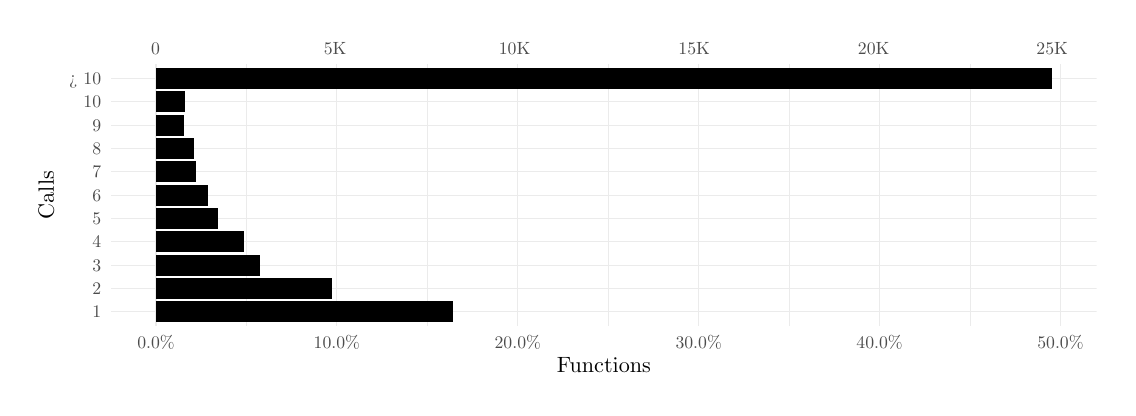
\begin{tikzpicture}[x=1pt,y=1pt]
\definecolor{fillColor}{RGB}{255,255,255}
\path[use as bounding box,fill=fillColor,fill opacity=0.00] (0,0) rectangle (390.26,130.09);
\begin{scope}
\path[clip] ( 30.17, 22.32) rectangle (386.26,116.83);
\definecolor{drawColor}{gray}{0.92}

\path[draw=drawColor,line width= 0.2pt,line join=round] ( 79.04, 22.32) --
	( 79.04,116.83);

\path[draw=drawColor,line width= 0.2pt,line join=round] (144.41, 22.32) --
	(144.41,116.83);

\path[draw=drawColor,line width= 0.2pt,line join=round] (209.77, 22.32) --
	(209.77,116.83);

\path[draw=drawColor,line width= 0.2pt,line join=round] (275.14, 22.32) --
	(275.14,116.83);

\path[draw=drawColor,line width= 0.2pt,line join=round] (340.51, 22.32) --
	(340.51,116.83);

\path[draw=drawColor,line width= 0.4pt,line join=round] ( 30.17, 27.38) --
	(386.26, 27.38);

\path[draw=drawColor,line width= 0.4pt,line join=round] ( 30.17, 35.82) --
	(386.26, 35.82);

\path[draw=drawColor,line width= 0.4pt,line join=round] ( 30.17, 44.26) --
	(386.26, 44.26);

\path[draw=drawColor,line width= 0.4pt,line join=round] ( 30.17, 52.70) --
	(386.26, 52.70);

\path[draw=drawColor,line width= 0.4pt,line join=round] ( 30.17, 61.14) --
	(386.26, 61.14);

\path[draw=drawColor,line width= 0.4pt,line join=round] ( 30.17, 69.58) --
	(386.26, 69.58);

\path[draw=drawColor,line width= 0.4pt,line join=round] ( 30.17, 78.01) --
	(386.26, 78.01);

\path[draw=drawColor,line width= 0.4pt,line join=round] ( 30.17, 86.45) --
	(386.26, 86.45);

\path[draw=drawColor,line width= 0.4pt,line join=round] ( 30.17, 94.89) --
	(386.26, 94.89);

\path[draw=drawColor,line width= 0.4pt,line join=round] ( 30.17,103.33) --
	(386.26,103.33);

\path[draw=drawColor,line width= 0.4pt,line join=round] ( 30.17,111.77) --
	(386.26,111.77);

\path[draw=drawColor,line width= 0.4pt,line join=round] ( 46.36, 22.32) --
	( 46.36,116.83);

\path[draw=drawColor,line width= 0.4pt,line join=round] (111.72, 22.32) --
	(111.72,116.83);

\path[draw=drawColor,line width= 0.4pt,line join=round] (177.09, 22.32) --
	(177.09,116.83);

\path[draw=drawColor,line width= 0.4pt,line join=round] (242.46, 22.32) --
	(242.46,116.83);

\path[draw=drawColor,line width= 0.4pt,line join=round] (307.82, 22.32) --
	(307.82,116.83);

\path[draw=drawColor,line width= 0.4pt,line join=round] (373.19, 22.32) --
	(373.19,116.83);
\definecolor{fillColor}{RGB}{0,0,0}

\path[fill=fillColor] ( 46.36,107.97) rectangle (370.07,115.57);

\path[fill=fillColor] ( 46.36, 23.58) rectangle (153.52, 31.18);

\path[fill=fillColor] ( 46.36, 99.53) rectangle ( 56.78,107.13);

\path[fill=fillColor] ( 46.36, 32.02) rectangle (109.88, 39.62);

\path[fill=fillColor] ( 46.36, 40.46) rectangle ( 83.98, 48.06);

\path[fill=fillColor] ( 46.36, 48.90) rectangle ( 78.12, 56.49);

\path[fill=fillColor] ( 46.36, 57.34) rectangle ( 68.81, 64.93);

\path[fill=fillColor] ( 46.36, 65.78) rectangle ( 65.03, 73.37);

\path[fill=fillColor] ( 46.36, 74.22) rectangle ( 60.74, 81.81);

\path[fill=fillColor] ( 46.36, 82.66) rectangle ( 60.20, 90.25);

\path[fill=fillColor] ( 46.36, 91.10) rectangle ( 56.47, 98.69);
\end{scope}
\begin{scope}
\path[clip] (  0.00,  0.00) rectangle (390.26,130.09);
\definecolor{drawColor}{gray}{0.30}

\node[text=drawColor,anchor=base,inner sep=0pt, outer sep=0pt, scale=  0.64] at ( 46.21,120.43) {0};

\node[text=drawColor,anchor=base,inner sep=0pt, outer sep=0pt, scale=  0.64] at (111.09,120.43) {5K};

\node[text=drawColor,anchor=base,inner sep=0pt, outer sep=0pt, scale=  0.64] at (175.96,120.43) {10K};

\node[text=drawColor,anchor=base,inner sep=0pt, outer sep=0pt, scale=  0.64] at (240.83,120.43) {15K};

\node[text=drawColor,anchor=base,inner sep=0pt, outer sep=0pt, scale=  0.64] at (305.70,120.43) {20K};

\node[text=drawColor,anchor=base,inner sep=0pt, outer sep=0pt, scale=  0.64] at (370.22,120.43) {25K};
\end{scope}
\begin{scope}
\path[clip] (  0.00,  0.00) rectangle (390.26,130.09);
\definecolor{drawColor}{gray}{0.30}

\node[text=drawColor,anchor=base east,inner sep=0pt, outer sep=0pt, scale=  0.64] at ( 26.57, 25.18) {1};

\node[text=drawColor,anchor=base east,inner sep=0pt, outer sep=0pt, scale=  0.64] at ( 26.57, 33.62) {2};

\node[text=drawColor,anchor=base east,inner sep=0pt, outer sep=0pt, scale=  0.64] at ( 26.57, 42.05) {3};

\node[text=drawColor,anchor=base east,inner sep=0pt, outer sep=0pt, scale=  0.64] at ( 26.57, 50.49) {4};

\node[text=drawColor,anchor=base east,inner sep=0pt, outer sep=0pt, scale=  0.64] at ( 26.57, 58.93) {5};

\node[text=drawColor,anchor=base east,inner sep=0pt, outer sep=0pt, scale=  0.64] at ( 26.57, 67.37) {6};

\node[text=drawColor,anchor=base east,inner sep=0pt, outer sep=0pt, scale=  0.64] at ( 26.57, 75.81) {7};

\node[text=drawColor,anchor=base east,inner sep=0pt, outer sep=0pt, scale=  0.64] at ( 26.57, 84.25) {8};

\node[text=drawColor,anchor=base east,inner sep=0pt, outer sep=0pt, scale=  0.64] at ( 26.57, 92.69) {9};

\node[text=drawColor,anchor=base east,inner sep=0pt, outer sep=0pt, scale=  0.64] at ( 26.57,101.13) {10};

\node[text=drawColor,anchor=base east,inner sep=0pt, outer sep=0pt, scale=  0.64] at ( 26.57,109.57) {> 10};
\end{scope}
\begin{scope}
\path[clip] (  0.00,  0.00) rectangle (390.26,130.09);
\definecolor{drawColor}{gray}{0.30}

\node[text=drawColor,anchor=base,inner sep=0pt, outer sep=0pt, scale=  0.64] at ( 46.36, 14.31) {0.0{\%}};

\node[text=drawColor,anchor=base,inner sep=0pt, outer sep=0pt, scale=  0.64] at (111.72, 14.31) {10.0{\%}};

\node[text=drawColor,anchor=base,inner sep=0pt, outer sep=0pt, scale=  0.64] at (177.09, 14.31) {20.0{\%}};

\node[text=drawColor,anchor=base,inner sep=0pt, outer sep=0pt, scale=  0.64] at (242.46, 14.31) {30.0{\%}};

\node[text=drawColor,anchor=base,inner sep=0pt, outer sep=0pt, scale=  0.64] at (307.82, 14.31) {40.0{\%}};

\node[text=drawColor,anchor=base,inner sep=0pt, outer sep=0pt, scale=  0.64] at (373.19, 14.31) {50.0{\%}};
\end{scope}
\begin{scope}
\path[clip] (  0.00,  0.00) rectangle (390.26,130.09);
\definecolor{drawColor}{RGB}{0,0,0}

\node[text=drawColor,anchor=base,inner sep=0pt, outer sep=0pt, scale=  0.80] at (208.22,  5.56) {Functions};
\end{scope}
\begin{scope}
\path[clip] (  0.00,  0.00) rectangle (390.26,130.09);
\definecolor{drawColor}{RGB}{0,0,0}

\node[text=drawColor,rotate= 90.00,anchor=base,inner sep=0pt, outer sep=0pt, scale=  0.80] at (  9.51, 69.58) {Calls};
\end{scope}
\end{tikzpicture}

  \caption{Call Distribution}
  \label{fig:callDist}
\end{figure}

We observe 137.2M calls to these functions. Figure ~\ref{fig:callDist} shows the
number of distribution of calls across functions called in the synthesis
phase. 49.5\% functions are called more than 10 times. 16.4\% functions are
called only once, leading to low coverage. These functions are spread across 414
packages.

We observe 294.45M arguments created in our execution traces. Of those 3.9M are
missing, 18.9M are $...$ arguments, and 271.6M are promises. These arguments
correspond to 185.9K parameter positions of the 50,435 functions for which we
generate signatures. Figure ~\ref{fig:paramDist} shows the distribution of these
parameters per function.

\begin{figure}[!h]
  \centering
  % Created by tikzDevice version 0.12.3.1 on 2021-04-09 22:35:57
% !TEX encoding = UTF-8 Unicode
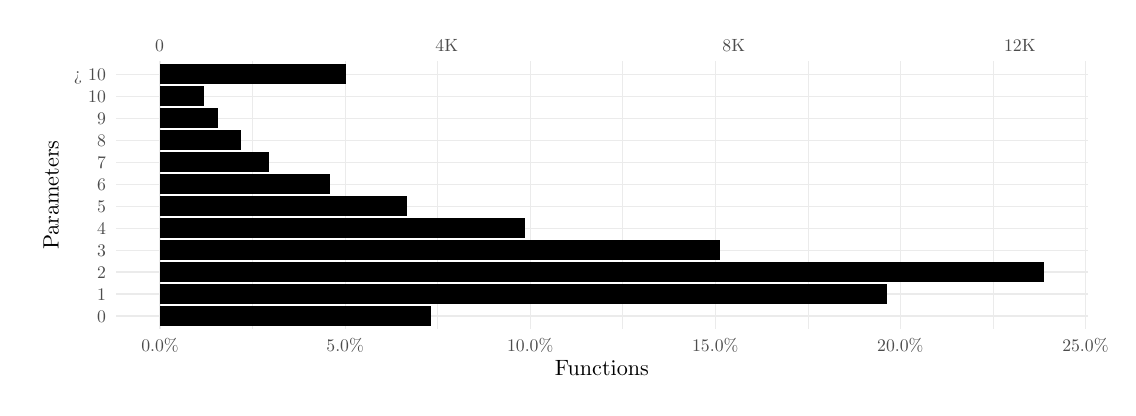
\begin{tikzpicture}[x=1pt,y=1pt]
\definecolor{fillColor}{RGB}{255,255,255}
\path[use as bounding box,fill=fillColor,fill opacity=0.00] (0,0) rectangle (390.26,130.09);
\begin{scope}
\path[clip] ( 31.86, 21.16) rectangle (383.14,117.99);
\definecolor{drawColor}{gray}{0.92}

\path[draw=drawColor,line width= 0.2pt,line join=round] ( 81.27, 21.16) --
	( 81.27,117.99);

\path[draw=drawColor,line width= 0.2pt,line join=round] (148.15, 21.16) --
	(148.15,117.99);

\path[draw=drawColor,line width= 0.2pt,line join=round] (215.02, 21.16) --
	(215.02,117.99);

\path[draw=drawColor,line width= 0.2pt,line join=round] (281.90, 21.16) --
	(281.90,117.99);

\path[draw=drawColor,line width= 0.2pt,line join=round] (348.77, 21.16) --
	(348.77,117.99);

\path[draw=drawColor,line width= 0.4pt,line join=round] ( 31.86, 25.92) --
	(383.14, 25.92);

\path[draw=drawColor,line width= 0.4pt,line join=round] ( 31.86, 33.86) --
	(383.14, 33.86);

\path[draw=drawColor,line width= 0.4pt,line join=round] ( 31.86, 41.80) --
	(383.14, 41.80);

\path[draw=drawColor,line width= 0.4pt,line join=round] ( 31.86, 49.73) --
	(383.14, 49.73);

\path[draw=drawColor,line width= 0.4pt,line join=round] ( 31.86, 57.67) --
	(383.14, 57.67);

\path[draw=drawColor,line width= 0.4pt,line join=round] ( 31.86, 65.61) --
	(383.14, 65.61);

\path[draw=drawColor,line width= 0.4pt,line join=round] ( 31.86, 73.54) --
	(383.14, 73.54);

\path[draw=drawColor,line width= 0.4pt,line join=round] ( 31.86, 81.48) --
	(383.14, 81.48);

\path[draw=drawColor,line width= 0.4pt,line join=round] ( 31.86, 89.42) --
	(383.14, 89.42);

\path[draw=drawColor,line width= 0.4pt,line join=round] ( 31.86, 97.35) --
	(383.14, 97.35);

\path[draw=drawColor,line width= 0.4pt,line join=round] ( 31.86,105.29) --
	(383.14,105.29);

\path[draw=drawColor,line width= 0.4pt,line join=round] ( 31.86,113.23) --
	(383.14,113.23);

\path[draw=drawColor,line width= 0.4pt,line join=round] ( 47.83, 21.16) --
	( 47.83,117.99);

\path[draw=drawColor,line width= 0.4pt,line join=round] (114.71, 21.16) --
	(114.71,117.99);

\path[draw=drawColor,line width= 0.4pt,line join=round] (181.58, 21.16) --
	(181.58,117.99);

\path[draw=drawColor,line width= 0.4pt,line join=round] (248.46, 21.16) --
	(248.46,117.99);

\path[draw=drawColor,line width= 0.4pt,line join=round] (315.34, 21.16) --
	(315.34,117.99);

\path[draw=drawColor,line width= 0.4pt,line join=round] (382.21, 21.16) --
	(382.21,117.99);
\definecolor{fillColor}{RGB}{0,0,0}

\path[fill=fillColor] ( 47.83,109.66) rectangle (115.04,116.80);

\path[fill=fillColor] ( 47.83, 22.35) rectangle (145.68, 29.50);

\path[fill=fillColor] ( 47.83, 30.29) rectangle (310.59, 37.43);

\path[fill=fillColor] ( 47.83,101.72) rectangle ( 63.63,108.86);

\path[fill=fillColor] ( 47.83, 38.23) rectangle (367.18, 45.37);

\path[fill=fillColor] ( 47.83, 46.16) rectangle (250.08, 53.31);

\path[fill=fillColor] ( 47.83, 54.10) rectangle (179.66, 61.24);

\path[fill=fillColor] ( 47.83, 62.04) rectangle (137.11, 69.18);

\path[fill=fillColor] ( 47.83, 69.97) rectangle (109.42, 77.12);

\path[fill=fillColor] ( 47.83, 77.91) rectangle ( 87.10, 85.05);

\path[fill=fillColor] ( 47.83, 85.85) rectangle ( 77.25, 92.99);

\path[fill=fillColor] ( 47.83, 93.78) rectangle ( 68.76,100.93);
\end{scope}
\begin{scope}
\path[clip] (  0.00,  0.00) rectangle (390.26,130.09);
\definecolor{drawColor}{gray}{0.30}

\node[text=drawColor,anchor=base,inner sep=0pt, outer sep=0pt, scale=  0.64] at ( 47.69,121.59) {0};

\node[text=drawColor,anchor=base,inner sep=0pt, outer sep=0pt, scale=  0.64] at (151.42,121.59) {4K};

\node[text=drawColor,anchor=base,inner sep=0pt, outer sep=0pt, scale=  0.64] at (255.15,121.59) {8K};

\node[text=drawColor,anchor=base,inner sep=0pt, outer sep=0pt, scale=  0.64] at (358.53,121.59) {12K};
\end{scope}
\begin{scope}
\path[clip] (  0.00,  0.00) rectangle (390.26,130.09);
\definecolor{drawColor}{gray}{0.30}

\node[text=drawColor,anchor=base east,inner sep=0pt, outer sep=0pt, scale=  0.64] at ( 28.26, 23.72) {0};

\node[text=drawColor,anchor=base east,inner sep=0pt, outer sep=0pt, scale=  0.64] at ( 28.26, 31.66) {1};

\node[text=drawColor,anchor=base east,inner sep=0pt, outer sep=0pt, scale=  0.64] at ( 28.26, 39.59) {2};

\node[text=drawColor,anchor=base east,inner sep=0pt, outer sep=0pt, scale=  0.64] at ( 28.26, 47.53) {3};

\node[text=drawColor,anchor=base east,inner sep=0pt, outer sep=0pt, scale=  0.64] at ( 28.26, 55.47) {4};

\node[text=drawColor,anchor=base east,inner sep=0pt, outer sep=0pt, scale=  0.64] at ( 28.26, 63.40) {5};

\node[text=drawColor,anchor=base east,inner sep=0pt, outer sep=0pt, scale=  0.64] at ( 28.26, 71.34) {6};

\node[text=drawColor,anchor=base east,inner sep=0pt, outer sep=0pt, scale=  0.64] at ( 28.26, 79.28) {7};

\node[text=drawColor,anchor=base east,inner sep=0pt, outer sep=0pt, scale=  0.64] at ( 28.26, 87.21) {8};

\node[text=drawColor,anchor=base east,inner sep=0pt, outer sep=0pt, scale=  0.64] at ( 28.26, 95.15) {9};

\node[text=drawColor,anchor=base east,inner sep=0pt, outer sep=0pt, scale=  0.64] at ( 28.26,103.09) {10};

\node[text=drawColor,anchor=base east,inner sep=0pt, outer sep=0pt, scale=  0.64] at ( 28.26,111.02) {> 10};
\end{scope}
\begin{scope}
\path[clip] (  0.00,  0.00) rectangle (390.26,130.09);
\definecolor{drawColor}{gray}{0.30}

\node[text=drawColor,anchor=base,inner sep=0pt, outer sep=0pt, scale=  0.64] at ( 47.83, 13.15) {0.0{\%}};

\node[text=drawColor,anchor=base,inner sep=0pt, outer sep=0pt, scale=  0.64] at (114.71, 13.15) {5.0{\%}};

\node[text=drawColor,anchor=base,inner sep=0pt, outer sep=0pt, scale=  0.64] at (181.58, 13.15) {10.0{\%}};

\node[text=drawColor,anchor=base,inner sep=0pt, outer sep=0pt, scale=  0.64] at (248.46, 13.15) {15.0{\%}};

\node[text=drawColor,anchor=base,inner sep=0pt, outer sep=0pt, scale=  0.64] at (315.34, 13.15) {20.0{\%}};

\node[text=drawColor,anchor=base,inner sep=0pt, outer sep=0pt, scale=  0.64] at (382.21, 13.15) {25.0{\%}};
\end{scope}
\begin{scope}
\path[clip] (  0.00,  0.00) rectangle (390.26,130.09);
\definecolor{drawColor}{RGB}{0,0,0}

\node[text=drawColor,anchor=base,inner sep=0pt, outer sep=0pt, scale=  0.80] at (207.50,  4.40) {Functions};
\end{scope}
\begin{scope}
\path[clip] (  0.00,  0.00) rectangle (390.26,130.09);
\definecolor{drawColor}{RGB}{0,0,0}

\node[text=drawColor,rotate= 90.00,anchor=base,inner sep=0pt, outer sep=0pt, scale=  0.80] at ( 11.20, 69.58) {Parameters};
\end{scope}
\end{tikzpicture}

  \caption{Parameter Distribution}
  \label{fig:paramDist}
\end{figure}

7.3\% functions have 0 parameters, 19.6\% have 1, and
5.0\% have over 10. There are 15 functions with over 50 parameters that come
from 10 packages. \emph{ComplexHeatmap::pheatmap} (51),
\emph{network::plot.network.default} (52), \emph{rpart.plot::get.layout} (53),
\emph{sna::gplot} (54), \emph{Hmisc::latex.default} (55),
\emph{VennDiagram::draw.quintuple.venn} (57) \emph{pROC::plot.roc.roc} (58),
\emph{rpart.plot::draw.node.numbers} (60), \emph{gplots::heatmap.2} (63),
\emph{Hmisc::event.chart} (66), \emph{ComplexHeatmap::Heatmap} (83),
\emph{ggplot2::theme} (95), \emph{ergm::control.ergm} (117),
\emph{rpart.plot::prp} (119), and
\emph{rpart.plot::check.if.dot.arg.supported.by.rpart.rules} (122) with the
highest number of parameters.

\section{Evaluation}

\OF{We probably need some proper research questions we list earlier, that go along with
the evaluation...}

In this section we test the following hypotheses:

\begin{itemize}
  \item[{\bf H1}] Most argument evaluations observed in R conform with strict semantics
  \item[{\bf H2}] Strict semantics does not break most programs
  \item[{\bf H3}] Strict semantics is beneficial for performance
\end{itemize}


% TODO for end
% Table~\cite{tab:ten_sigs} shows ten representative signatures generated by the
% synthesis step of our experiments.
%
% \begin{table}
%   \vspace{-3mm}
%   \caption{Strictness Signatures} \label{table:ten_sigs}
%   \centering
%   \begin{tabular}{ll}
%     \toprule
%     \bf Function &\bf Strictness Signature\\
%     \hline
%     \bottomrule
%   \end{tabular}
% \end{table}

\subsection{Strictness (H1)}

This part of evaluation sheds light on the strictness of functions in our
corpus. Conceptually, a function is strict if it evaluates all of its argument
in a single pre-ordained order~\cite{oopsla19b} across all calls.
Figure~\ref{fig:force_order} shows the number of evaluation orders of the
functions in our corpus. XX(XX\%) functions have a single evaluation order. Out
of those, XX functions evaluate all of their arguments. Evaluation orders
greater than 5 are rare and are found only in XX functions.


\subsubsection{...}

\subsubsection{Metaprogramming}
There are XX $...$ parameters which make XXX functions non-strict. R's
metaprogramming support introduces another source of laziness. XX parameters are
metaprogrammed in our corpus.

\subsubsection{Unevaluated Arguments}
Of the 294.45M total arguments in our corpus, 30.4M argument promises were not
evaluated. They correspond to 52,083 parameters of 26,398 functions from 473
packages. These functions are non-strict in the corresponding parameters.

Based on argument evaluation, we can classify parameter positions into three
categories.\always parameters are those whose arguments are evaluated in all
calls. \sometimes parameters are those whose arguments are evaluated at least
once but not always. \never parameters are those whose arguments are never
evaluated. Table~\ref{table:argeval} shows the number and proportion of
parameters that belong to these categories.

\begin{table}[!h]
  \vspace{-3mm}
  \caption{Argument Evaluation}\label{table:argeval}
  \vspace{-3mm}
  \begin{tabular}{lr|lr|lr}
    \toprule
    \textbf{Type}&\multicolumn{2}{c}{\textbf{Parameters}}&\multicolumn{2}{c}{\textbf{Functions}}&\textbf{Packages}\\
    \midrule
    Always&144565&73.51\%&48456&96.08\%&490\\
    Sometimes&16411&8.35\%&7070&14.02\%&410\\
    Never&10637&5.41\%&5907&11.71\%&405\\
    \midrule
    Sometimes*&15130&7.69\%&6609&13.1\%&406\\
    Never*&9251&4.7\%&5121&10.15\%&400\\
    \bottomrule
  \end{tabular}
\end{table}

Majority of parameters are \always parameters, suggesting that arguments passed
to functions are evaluated in most of the cases. This is followed by 8.35\%
\sometimes parameters. Their presence indicates use of metaprogramming or
unexplored control flow paths in the function. Lastly, we have 5.41\% \never
arguments whose presence indicates lack of coverage, metaprogramming, or dummy
parameter. The \textbf{Functions} field gives the number of functions with
\always, \sometimes, and \never arguments. The same function can appear in
multiple columns since different parameters can have different evaluation
classification. The \textbf{Packages} field of Table~\ref{table:areval} tells us
that \never and \sometimes functions are spread across many packages.


\sometimesStar and \neverStar in Table~\ref{table:argeval} are the number of
\sometimes and \never cases without metaprogrammed. The different is small which
suggests that metaprogramming is not the primary reason for arguments remaining
unevaluated. Turning to the number of calls, we find that 78.33\% of functions
with \never parameters are called more than once. This suggests that a lack of
call diversity could be one of factors for \never arguments' existence. With
better call diversity, the \never parameters will turn into \sometimes.

\paragraph{Qualitative Analysis}

We analyzed a sample of functions with \sometimes and \never parameters to
identify usage patterns.

First, we look at \sometimes parameters. A common patter occurring in 30
packages is the following definition of \code{\%||\%} function.

\begin{lstlisting}
lazyeval::\%||\% <- function(x, y) if(is.null(x)) y else x
\end{lstlisting}

This function evaluates its second argument \code{y} only if \code{x} is
\code{NULL}. This makes \code{y} a \sometimes parameter. This pattern suggests
that \code{y} is a \sometimes parameter for a reason and should not be evaluated
unless needed. However, there are other functions with multiple paths where
evaluating the \sometimes argument is expected to be benign. For example, in
\code{bayesplot::is_whole_number} function, the \code{tol} argument is only
evaluated when \code{x} is a numeric value. I

\begin{lstlisting}
bayesplot::is_whole_number <- function(x, tol = .Machine$double.eps) {
    if (!is.numeric(x)) { FALSE } else { abs(x - round(x)) < tol }
}
\end{lstlisting}


Another pattern occurring in 4 packages is the definition of
\code{on_package_load}.

\begin{lstlisting}
glue::on_package_load <- function(pkg, expr) {
    if (isNamespaceLoaded(pkg)) { expr }
    else {
        thunk <- function(...) expr
        setHook(packageEvent(pkg, "onLoad"), thunk)
    }
}
\end{lstlisting}

Here, if package \code{pkg} is not loaded, the \code{expr} argument's evaluation
is delayed until the package's \code{onLoad} event occurs. In some executions,
we see the \code{expr} argument being evaluated if package \code{pkg} is loaded
and in other iterations, we don't. The way this code is written suggests that
\code{expr} should not be evaluated strictly.

S3 generics result in many \sometimes and \never parameters. These functions
dynamically dispatch to a specific implementation with the same name based on
the first argument's class. In this case, the first argument is always evaluated
but the remaining arguments might not be needed by the specific method. Across
all executions, we observed that \code{n} and \code{m} are evaluated sometimes
but \code{r} is never evaluated.

\begin{lstlisting}
abind::acorn <- function(x, n=6, m=5, r=1, ...) UseMethod('acorn')
\end{lstlisting}


Next, we turn our attention to \never parameters.

The most common case is when an argument is not used in some branch of the
function. Due to lack of call diversity, the branch in which the argument is
used is never taken and the parameter is classified as \never. For example,
\code{discretize} function of package \code{actuar} only uses \code{xlim} if
\code{from} and \code{to} parameters are missing.
\begin{lstlisting}
actuar:::discretize <- function (cdf, from, to, ..., xlim = NULL) {
    ...
    if (missing(from)) from <- xlim[1];
    if (missing(to)) to <- xlim[2];
    ...
}
\end{lstlisting}


Another pattern leading to \never parameters is when a function is called with a
certain interface even if it does not use those arguments. R calls a package's
\code{.onLoad} function with arguments \code{libname} and \code{pkgname} when
the package is loaded. The \code{.onLoad} hook of \code{assertive.base} package
ignores them.
\begin{lstlisting}
assertive.base::.onLoad <- function(libname, pkgname) {
    options(assertive.severity = "stop")
}
\end{lstlisting}

The \code{proxy} package defines over a dozen methods with the interface
\code{function(a, b, c, d, n) ...} that implement different proximity metrics by
using only a subset of the arguments.
This also happens in method dispatch when the generic method defines a parameter
which is not used by the specific method. For example \code{bit64} package
defines \code{unipos} generic method with a parameter \code{incomparables} which
is not used by its only concrete implementation \code{unipos.integer64}


Sometimes arguments don't need to be used by design.
The \code{tail} operation in package \code{dbplyr} is not defined for
\code{tbl_lazy} objects. So the function throws an error when called without
using any of its arguments.
\begin{lstlisting}
dbplyr::tail.tbl_lazy <- function(x, n = 6L, ...) {
    stop("tail() is not supported by sql sources", call. = FALSE)
}
\end{lstlisting}

Sometimes packages implement a specialized compatible wrapper.
\code{jsonlite} package implements \code{stop} function with the same interface
as R's \code{base} package's \code{stop} function but ignores its \code{call.}
argument.
\begin{lstlisting}
jsonlite::stop <- function(..., call. = FALSE) {
    base::stop(..., call. = FALSE)
}
\end{lstlisting}

\never parameters can also represent an erroneous condition that would not
happen in a correct program. In \code{codetools} package, function
\code{checkSymOrString} fails if the argument does not have the correct type. In
all the calls we observed, the \code{signal} argument was not used because
\code{e} had the correct type.
\begin{lstlisting}
codetools::checkSymOrString <- function(e, signal = stop) {
    type <- typeof(e)
    if (type == "symbol" || type == "character") e
    else signal("not a symbol or string")
}
\end{lstlisting}

\subsubsection{Reflection}

R allows reflective access to parent scope through \code{as.environment} and
\code{pos.to.env} functions when called with argument \code{-1}.
They return the environment of the caller with respect to call in which they are

evaluated. Consider the following example in which function f is called with the
same argument \code{as.environment(-1)} for both \code{x} and \code{y}
parameters. The first argument \code{x} is evaluated immediately inside
function \code{f} and the second argument \code{y} is evaluated inside the
\code{id} function. \code{x} evaluates to the environment of the parent of
\code{f} which is the \code{global} environment, whereas \code{y} evaluates to
the environment of \code{f} which is the parent of \code{id} inside of which
\code{y} is evaluated.

\begin{lstlisting}
id <- function(a) a
f <- function(x, y) { x; id(y); }
f(x = as.environment(-1), y = as.environment(-1))
\end{lstlisting}

There are two points to note here. First, the strictness of \code{f} with
respect to \code{x} and \code{y} depends on how \code{f} is called. Second,
\code{f} will now be lazy in argument \code{y}, otherwise we will end up
evaluating inside \code{f}. Erroneously evaluating \code{y} strictly would
result in an incorrect environment, but not an error, which could turn into a
debugging nightmare.

\code{as.environment} is internally implemented using \code{pos.to.env} so the
two functions have same semantics when called with \code{-1} as the argument.

It is interesting to note that there are other functions providing reflective
access to call stack frames such as \code{parent.frame}, \code{sys.frame}, etc.
However, these take into account the current evaluation environment to identify
the parent caller. A promise evaluates the argument expression inside the
caller's environment. So, a call to \code{parent.frame()} directly inside the
argument will use the caller's environment to identify the parent dynamic scope.
This makes its result independent of the point at which the promise is
evaluated.

Another wrinkle introduced by this setup is that it can transitively affect the
strictness of other function arguments. Imagine \code{f} is called from \code{g}
as shown below.

\begin{lstlisting}
g <- function(u, v) {
    f(u, v)
}
g(as.environment(-1), as.environment(-1))
\end{lstlisting}

Clearly, in this case we have to make \code{g} non-strict in \code{u} and
\code{v}. Their results depend upon how they are evaluated inside \code{f}.

We identified 2710 arguments which directly call \code{as.environment(-1)} and
\code{pos.to.env(-1)} in our corpus. They correspond to 2 parameters from 2
functions, \code{R.oo::.getFunctionByName}, and \code{backports:::get0}.

\code{R.oo:::.getFunctionByName} is a private function of \code{R.oo} package
which searches for a function by name in different scopes, configured by its
arguments. Its fourth parameter, \code{callEnvir}, has a default value of
\code{as.environment(-1)}. It is called 2707 times. The relevant part of its
definition is that \code{callEnvir} is evaluated by assigning it to
\code{envirT} before it is passed down to the \code{exists} function.

\begin{lstlisting}
function(name, where = c("ns", "search", "ns*"),
         envir = NULL, callEnvir = as.environment(-1L),
         class = "function", mustExist = TRUE, ...) {
    ...
    envirT <- callEnvir
    if (exists(name, mode = "function", envir = envirT, inherits = TRUE))
    ...
}
\end{lstlisting}

\code{backports::get0} is a private function of \code{backports} package which
looks up a variable in a scope, similar in spirit to
\code{R.oo:::.getFunctionByName}. This function is called 3 times, always with
the default value \code{pos.to.env(-1)} for \code{envir} argument. Unlike
\code{R.oo:::.getFunctionByName}, \code{backports:::get0} passes \code{envir}
unevaluated to \code{mget}. \code{mget} in turn evaluates \code{envir} and looks
up variable referred to by \code{x} in \code{envir}. Clearly, with the default
value of \code{envir}, lookup will happen in the environment of
\code{backports::get0} which only has bindings for its parameters. What makes
this work is that it is only called from the top-level, with the argument
\code{inherits} set to \code{TRUE}. This causes \code{mget} to search
recursively in enclosing scopes beginning from \code{envir} until lookup
succeeds in the \code{global} environment used for top-level bindings.

\begin{lstlisting}
function (x, envir = pos.to.env(-1L), mode = "any",
          inherits = TRUE, ifnotfound = NULL)  {
    ....
    mget(x[1L], envir = envir, mode = mode,
         inherits = inherits, ifnotfound = list(ifnotfound))[[1L]]
}
\end{lstlisting}

Calls to \code{R.oo:::.getFunctionByName} result in transitively making 1821
argument lazy. They correspond to 18 parameters from 15 functions of 3 packages.
We manually analyzed these cases but found that none of these functions pass
their arguments containing calls to \code{as.environment(-1)} or
\code{pos.to.env(-1)} to \code{R.oo:::.getFunctionByName}. They are identified
as lazy because our dynamic analyzer is conservative. When a reflective call
happens from an argument promise, it taints all the function arguments on the
stack. This has the effect of making more arguments lazy than needed.

\code{backports::get0} is invoked from the top-level so it does not result in
spurious transitive laziness.

\subsubsection{Side-Effects}

\subsection{Robustness (H2)} \label{Evaluation:Robustness}

\begin{table}
  \vspace{-3mm}
  \small
  \caption{Strictness Distribution} \label{table:strictdist}
  \centering
  \begin{tabular}{lcccr|lr|lr}
    \toprule
    \#&\bf Unevaluted & \bf Side-Effecting & \bf Reflective & \multicolumn{2}{c}{\textbf{Parameters}} & \multicolumn{2}{c}{\textbf{Functions}}& \bf Packages\\
    \midrule
    0&\xmark{}&\xmark{}&\xmark{}&128305&65.25\%&44377&85.93\%&489\\
    1&\xmark{}&\xmark{}&\cmark{}&134&0.07\%&124&0.24\%&47\\
    2&\xmark{}&\cmark{}&\xmark{}&7871&4\%&5805&11.24\%&399\\
    3&\xmark{}&\cmark{}&\cmark{}&408&0.21\%&385&0.75\%&93\\
    4&\cmark{}&\xmark{}&\xmark{}&27050&13.76\%&11333&21.95\%&453\\
    5&\cmark{}&\xmark{}&\cmark{}&13&0.01\%&12&0.02\%&11\\
    6&\cmark{}&\cmark{}&\xmark{}&1213&0.62\%&813&1.57\%&199\\
    7&\cmark{}&\cmark{}&\cmark{}&25&0.01\%&24&0.05\%&15\\
    \bottomrule
  \end{tabular}
\end{table}

\subsection{Performance (H3)}

Our main hypothesis regarding performance is that eager semantics lead to faster
execution of R programs. This hypothesis might seem
unexpected to some readers, as call-by-need is sometimes used to avoid
unnecessary computation in a program. On the other hand, delaying computations
is more complex to implement and we observed it to obstruct performance
in two ways: First, it leads to more allocations of promises used to represent
the delayed computation. Second, in combination with effects potentially
originating from promises, it obstructs more advanced compiler analysis and
optimizations. Especially the later point means that we expect the hypothesis to
hold even for a just-in-time compiler, that uses advanced optimizations.
To evaluate the hypothesis we extend the Ř virtual machine for R, such that all
promises are inlined at the call-site. In the following we call this modified
implementation Ř-strict. We evaluate the effects on the Ř benchmark
suite. As predicted by (H2) only a handful of functions, such as
\lstinline{tryCatch} had to be kept lazy for all the benchmarks to compute the
correct results. Based on the observations so far we pose the following predictions:

\begin{itemize}
  \item[{\bf H3.1}] Eager semantics improves performance of almost all benchmarks
    in the Ř suite.
  \item[{\bf H3.2}] A significant portion of the speedup is due to reduced
    garbage collection pressure.
  \item[{\bf H3.3}] Another significant portion of the speedup is due to improved
    compiler optimizations.
\end{itemize}

\paragraph{Speedup (H3.1)}

To evaluate the effect of eager semantics on performance we use the Ř virtual
machine and its benchmark suite. We implement a mode where all possible promises
are inlined in the first-tier compiler of Ř. Overal we observe a mean speedup of
\speedupRshStrict, ranging from \speedupRshStrictMin to \speedupRshStrictMax.

\paragraph{GC Pressure (H3.2)}

Even an optimizing compiler has to allocate many promises for R
code. We measure the number of promises allocated in the Ř benchmark suite
in GNU R, in Ř and in Ř-strict. The first step from a naive interpreter to an
optimizing compiler leads to an \promiseAlocationReductionGnurRsh
reduction in allocations. The second step
from lazy to eager semantics leads to \promiseAlocationReductionRshStrictToZero
benchmarks not allocating any promises at all. On the remainder we see an additional
\promiseAlocationReductionRshStrict reduction.
Overal, \promiseAlocationReductionRshStrictToZero benchmarks reduce to zero
allocations, the rest reduce on average by \promiseAlocationReductionGnurRshStrict.
Surprisingly the number of remaining promises is
still relatively high in some cases. The lowest reduction observed is
\promiseAlocationReductionGnurRshStrictMin.
\OF{TODO: where do they come from?} Also, overall xx\% of the
speedup reported in (H3.2) is attributed to shorter GC pauses.

\paragraph{Compiler Optimizations (H3.3)}

Our intuition is that inlining promises leads to code that is easier to analyze.
Therefore we expect an optimizing compiler to provide performance gains that go
beyond what can be explained by the reduction in GC pressure. We compare the
speedup of Ř-strict from (H3.1), with the same configuration, but having the
optimizing compiler disabled. Thhus all code is executed by the first-tier
bytecode interpreter. In this configuration the speedup is xx\%.




\section{Discussion}



\section{Migration Strategy}
- py2to3 does not do a good job
- hack has a simple migration tool
- scala 2 to 3 has migration tools

- If we have signatures for every test on CRAN.
-


%%\section*{Acknowledgments}
%% TODO: Thank Flip
\bibliography{bib/jv, bib/aviral}

\end{document}
